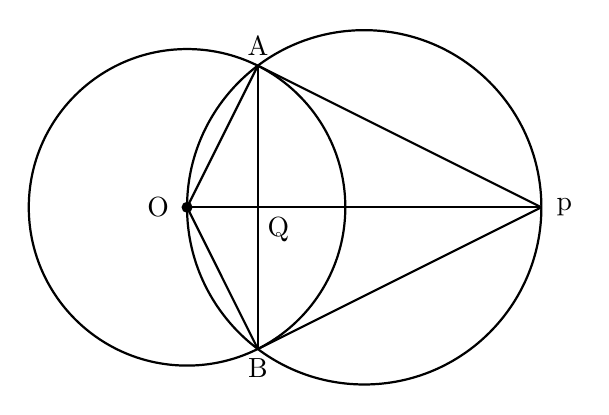
\begin{tikzpicture}[scale=1]

    % --- Coordinates ---
    % Q is the intersection of chord AB and the line of centers.
    \coordinate (Q) at (0,0);
    \coordinate (A) at (0,1.8);
    \coordinate (B) at (0,-1.8);
    \coordinate (O) at (-0.9,0); % Center of left circle
    
    % Right circle center (C) calculated so the circle passes through O and A.
    % p is the point on the right circumference.
    \coordinate (C) at (1.35,0); 
    \coordinate (p) at (3.6,0); 

    % --- Circles ---
    % Left circle centered at O with radius OA (~2.01cm)
    \draw[thick] (O) circle (2.01cm);
    
    % Right circle centered at C with radius CO (2.25cm). 
    % This ensures the circle passes exactly through point O.
    \draw[thick] (C) circle (2.25cm);

    % --- Line Segments (Exactly as shown in Fig 24) ---
    \draw[thick] (O) -- (p);      % Horizontal line from O to p
    \draw[thick] (A) -- (B);      % Common chord AB
    \draw[thick] (O) -- (A);      % Radius OA
    \draw[thick] (O) -- (B);      % Radius OB
    \draw[thick] (p) -- (A);      % Line from p to A
    \draw[thick] (p) -- (B);      % Line from p to B

    % --- Points ---
    % Only point O is explicitly marked with a dot in Fig 24
    \fill (O) circle (2pt);

    % --- Labels ---
    \node[above] at (A) {A};
    \node[below] at (B) {B};
    \node[left=3pt] at (O) {O};
    \node[below right] at (Q) {Q};
    \node[right=2pt] at (p) {p}; % Labeled with lowercase 'p' as in source

\end{tikzpicture}